% Шаблон (версия от 15.02.2016) предназначен 
% для использования студентами каф. ПМиИ СамГТУ 
% при оформлении отчетов по лабораторным работам. 
% Для настройки пакета listigs использовался материал 
% статьи Михаила Конника aka virens
% <http://mydebianblog.blogspot.ru/2012/12/latex.html>
% Copyright (c) 2016 by Mikhail Saushkin (msaushkin@gmail.com) 
% All rights reserved except the rights granted by the
% Creative Commons Attribution 4.0 International Licence
% <https://creativecommons.org/licenses/by/4.0/>
% Свежая версия шаблона здесь <https://www.overleaf.com/read/sqvxbnhgxxdm>
\documentclass[14pt,a4paper,report]{ncc}
\usepackage[a4paper, mag=1000, left=2.5cm, right=1cm, top=2cm, bottom=2cm, headsep=0.7cm, footskip=1cm]{geometry}
\usepackage[utf8]{inputenc}
\usepackage[english,russian,ukrainian]{babel}
\usepackage{indentfirst}
\usepackage[dvipsnames]{xcolor}
\usepackage[colorlinks]{hyperref}
\usepackage{listings} 
\usepackage{longtable}
\usepackage{caption}
\DeclareCaptionFont{white}{\color{white}} 
\DeclareCaptionFormat{listing}{\colorbox{gray}{\parbox{\textwidth}{#1#2#3}}}
\captionsetup[lstlisting]{format=listing,labelfont=white,textfont=white}

\lstset{% Собственно настройки вида листинга
inputencoding=utf8, extendedchars=\true, keepspaces = true, % поддержка кириллицы и пробелов в комментариях
% language=Pascal,            % выбор языка для подсветки (здесь это Pascal)
basicstyle=\small\sffamily, % размер и начертание шрифта для подсветки кода
backgroundcolor=\color{white}, % цвет фона подсветки - используем \usepackage{color}
showspaces=false,           % показывать или нет пробелы специальными отступами
showstringspaces=false,     % показывать или нет пробелы в строках
showtabs=false,             % показывать или нет табуляцию в строках
tabsize=4,                  % размер табуляции по умолчанию равен 2 пробелам
breaklines=true,            % автоматически переносить строки (да\нет)
breakatwhitespace=false,    % переносить строки только если есть пробел
escapeinside={\%*}{*)}      % если нужно добавить комментарии в коде
}

\begin{document}
% Переоформление некоторых стандартных названий
\renewcommand{\chaptername}{Лабораторна робота}
\def\contentsname{Зміст}

% Оформление титульного листа
\begin{titlepage}
\begin{center}
\textsc{МІНІСТЕРСТВО ОСВІТИ І НАУКИ УКРАЇНИ\\[2mm]
НАЦІОНАЛЬНИЙ ТЕХНІЧНИЙ УНІВЕРСИТЕТ УКРАЇНИ\\[2mm]
“КИЇВСЬКИЙ ПОЛІТЕХНІЧНИЙ ІНСТИТУТ\\[2mm]
iменi ІГОРЯ СІКОРСЬКОГО”}

\vfill

\textbf{Звіт з лабораторних робіт\\[3mm]
курс «Криптографія»\\[6mm]
\\[20mm]
}
\end{center}

\hfill
\begin{minipage}{.5\textwidth}
Виконав студент:\\[2mm] 
Костюковець Остап Юрійович\\
група: ФБ-96\\[5mm]

%Проверил:\\[2mm] 
%к.ф.-м.н., доцент\\
%Саушкин Михаил Николаевич

\end{minipage}%
\vfill
\begin{center}
 Київ, \theyear\ р.
\end{center}
\end{titlepage}

% Содержание
%\tableofcontents
\newpage

\chapter{Експериментальна оцінка ентропії на символ джерела
відкритого тексту}

\section{Мета роботи}
Засвоєння понять ентропії на символ джерела та його надлишковості, вивчення та
порівняння різних моделей джерела відкритого тексту для наближеного визначення
ентропії, набуття практичних навичок щодо оцінки ентропії на символ джерела.

\section{Завдання}
0. Уважно прочитати методичні вказівки до виконання комп’ютерного практикуму.

1. Написати програми для підрахунку частот букв і частот біграм в тексті, а також
підрахунку H 1 та H 2 за безпосереднім означенням. Підрахувати частоти букв та біграм, атакож значення H 1 та H 2 на довільно обраному тексті російською мовою достатньої
довжини (щонайменше 1Мб), де імовірності замінити відповідними частотами. Також
одержати значення H 1 та H 2 на тому ж тексті, в якому вилучено всі пробіли.

2. За допомогою програми CoolPinkProgram оцінити значення H ( 10 ) , H ( 20 ) , H ( 30 ) .

3. Використовуючи отримані значення ентропії, оцінити надлишковість російської
мови в різних моделях джерела.

\section{Хід роботи}

%\subsection{Лістинг програми}

\begin{table}[]
\centering
\caption{Ентропія, надлишковість}
\label{tab:my-table}
\begin{tabular}{ll}
\hline
\multicolumn{1}{|l|}{H1 (no spaces)}              & \multicolumn{1}{l|}{4.492315117172669}   \\ \hline
\multicolumn{1}{|l|}{H1 redundancy (no spaces)}   & \multicolumn{1}{l|}{0.10153697656546612} \\ \hline
\multicolumn{1}{|l|}{H2 (no spaces)}              & \multicolumn{1}{l|}{4.1802847959379115}  \\ \hline
\multicolumn{1}{|l|}{H2 redundancy (no spaces)}   & \multicolumn{1}{l|}{0.16394304081241773} \\ \hline
\multicolumn{1}{|l|}{H1 (with spaces)}            & \multicolumn{1}{l|}{4.406442333151592}   \\ \hline
\multicolumn{1}{|l|}{H1 redundancy (with spaces)} & \multicolumn{1}{l|}{0.11871153336968165} \\ \hline
\multicolumn{1}{|l|}{H2 (with spaces)}            & \multicolumn{1}{l|}{2.9080400719491637}  \\ \hline
\multicolumn{1}{|l|}{H2 redundancy (with spaces)} & \multicolumn{1}{l|}{0.4183919856101672}  \\ \hline
\multicolumn{1}{|l|}{H10}                         & \multicolumn{1}{l|}{3.1173 < R < 3.6639}  \\ \hline
\multicolumn{1}{|l|}{H20}                         & \multicolumn{1}{l|}{2.375 < R < 2.7555}  \\ \hline
\multicolumn{1}{|l|}{H30}                         & \multicolumn{1}{l|}{2.56079 < R < 3.0895}  \\ \hline
\end{tabular}
\end{table}


\subsection{Аналіз частот символів}

\begin{table}[]
\centering
\caption{H1 (no spaces)}
\label{tab:my-table}

\begin{tabular}{|l|l|}
\hline
\multicolumn{1}{|c|}{\textbf{о}} & \multicolumn{1}{c|}{\textbf{0.10584822334367971}} \\ \hline
е                                & 0.08399778970225735                               \\ \hline
а                                & 0.0824350401264014                                \\ \hline
н                                & 0.06483252245912892                               \\ \hline
и                                & 0.062443069723669614                              \\ \hline
т                                & 0.06075944449001265                               \\ \hline
л                                & 0.052529107290097264                              \\ \hline
р                                & 0.04690191372068225                               \\ \hline
с                                & 0.04619608621887991                               \\ \hline
в                                & 0.04187478145249371                               \\ \hline
к                                & 0.0377779600505951                                \\ \hline
д                                & 0.03151616927772478                               \\ \hline
у                                & 0.03098086279317743                               \\ \hline
м                                & 0.029899457354636227                              \\ \hline
п                                & 0.027291996736357238                              \\ \hline
я                                & 0.02227997392539382                               \\ \hline
ь                                & 0.022161256761482107                              \\ \hline
ы                                & 0.019676830294893435                              \\ \hline
г                                & 0.019454505424295145                              \\ \hline
з                                & 0.017880963378992674                              \\ \hline
б                                & 0.01760683465505109                               \\ \hline
ч                                & 0.015431072814632862                              \\ \hline
й                                & 0.011353677857737984                              \\ \hline
ж                                & 0.010216151578074883                              \\ \hline
ш                                & 0.009704588526309881                              \\ \hline
х                                & 0.008452662070513678                              \\ \hline
ю                                & 0.0071014448958095                                \\ \hline
щ                                & 0.00427813488860013                               \\ \hline
э                                & 0.004193953626917282                              \\ \hline
ц                                & 0.0033564579978674083                             \\ \hline
ф                                & 0.0013792775952651277                             \\ \hline
ъ                                & 0.00018778896836943055                            \\ \hline
\end{tabular}
\end{table}


% Please add the following required packages to your document preamble:
% Note: It may be necessary to compile the document several times to get a multi-page table to line up properly

\begin{table}[]
\centering
\caption{H2 (no spaces)}
\label{tab:my-table}
\begin{tabular}{ll}
\hline
\multicolumn{1}{|c|}{\textbf{то}} & \multicolumn{1}{c|}{\textbf{0.014304339004416279}} \\ \hline
\multicolumn{1}{|l|}{на}          & \multicolumn{1}{l|}{0.012314207638478175}          \\ \hline
\multicolumn{1}{|l|}{не}          & \multicolumn{1}{l|}{0.011584636703893491}          \\ \hline
\multicolumn{1}{|l|}{ст}          & \multicolumn{1}{l|}{0.010900394140984187}          \\ \hline
\multicolumn{1}{|l|}{по}          & \multicolumn{1}{l|}{0.010889601671537668}          \\ \hline
\multicolumn{1}{|l|}{ал}          & \multicolumn{1}{l|}{0.010874492214312541}          \\ \hline
\multicolumn{1}{|l|}{но}          & \multicolumn{1}{l|}{0.01060683897203887}           \\ \hline
\multicolumn{1}{|l|}{ко}          & \multicolumn{1}{l|}{0.010501072771462984}          \\ \hline
\multicolumn{1}{|l|}{ра}          & \multicolumn{1}{l|}{0.010036996585262668}          \\ \hline
\multicolumn{1}{|l|}{ен}          & \multicolumn{1}{l|}{0.009972241768583552}          \\ \hline
\multicolumn{1}{|l|}{он}          & \multicolumn{1}{l|}{0.009408874863475261}          \\ \hline
\multicolumn{1}{|l|}{ов}          & \multicolumn{1}{l|}{0.009331169083460324}          \\ \hline
\multicolumn{1}{|l|}{ер}          & \multicolumn{1}{l|}{0.00923187836455235}           \\ \hline
\multicolumn{1}{|l|}{от}          & \multicolumn{1}{l|}{0.008839032476699059}          \\ \hline
\multicolumn{1}{|l|}{ка}          & \multicolumn{1}{l|}{0.008672828447222666}          \\ \hline
\multicolumn{1}{|l|}{ро}          & \multicolumn{1}{l|}{0.008627500075547287}          \\ \hline
\multicolumn{1}{|l|}{ос}          & \multicolumn{1}{l|}{0.008349054363827097}          \\ \hline
\multicolumn{1}{|l|}{го}          & \multicolumn{1}{l|}{0.00828861653492659}           \\ \hline
\multicolumn{1}{|l|}{ол}          & \multicolumn{1}{l|}{0.008228178706026084}          \\ \hline
\multicolumn{1}{|l|}{ни}          & \multicolumn{1}{l|}{0.008143997444343236}          \\ \hline
\multicolumn{1}{|l|}{ак}          & \multicolumn{1}{l|}{0.007850442275397919}          \\ \hline
\multicolumn{1}{|l|}{ла}          & \multicolumn{1}{l|}{0.007833174324283487}          \\ \hline
\multicolumn{1}{|l|}{ло}          & \multicolumn{1}{l|}{0.007546094637006083}          \\ \hline
\multicolumn{1}{|l|}{во}          & \multicolumn{1}{l|}{0.007457596387544627}          \\ \hline
\multicolumn{1}{|l|}{пр}          & \multicolumn{1}{l|}{0.007306501815293361}          \\ \hline
\multicolumn{1}{|l|}{ор}          & \multicolumn{1}{l|}{0.007228796035278424}          \\ \hline
\multicolumn{1}{|l|}{ре}          & \multicolumn{1}{l|}{0.007058275018023424}          \\ \hline
\multicolumn{1}{|l|}{ет}          & \multicolumn{1}{l|}{0.00699352020134431}           \\ \hline
\multicolumn{1}{|l|}{ве}          & \multicolumn{1}{l|}{0.006790621775749753}          \\ \hline
\multicolumn{1}{|l|}{ел}          & \multicolumn{1}{l|}{0.006699965032398994}          \\ \hline
\multicolumn{1}{|l|}{ли}          & \multicolumn{1}{l|}{0.00656182142348355}           \\ \hline
\multicolumn{1}{|l|}{од}          & \multicolumn{1}{l|}{0.00649922510069374}           \\ \hline
\end{tabular}
\end{table}


\begin{table}[]
\centering
\caption{H1 (with spaces)}
\label{tab:my-table}
\begin{tabular}{ll}
\hline
\multicolumn{1}{|l|}{}  & \multicolumn{1}{l|}{0.16067119346633524}    \\ \hline
\multicolumn{1}{|c|}{о} & \multicolumn{1}{l|}{0.0888414629727595}     \\ \hline
\multicolumn{1}{|l|}{е} & \multicolumn{1}{l|}{0.07050176458226141}    \\ \hline
\multicolumn{1}{|l|}{а} & \multicolumn{1}{l|}{0.06919010384584726}    \\ \hline
\multicolumn{1}{|l|}{н} & \multicolumn{1}{l|}{0.05441580370018769}    \\ \hline
\multicolumn{1}{|l|}{и} & \multicolumn{1}{l|}{0.05241026718746603}    \\ \hline
\multicolumn{1}{|l|}{т} & \multicolumn{1}{l|}{0.05099715202945077}    \\ \hline
\multicolumn{1}{|l|}{л} & \multicolumn{1}{l|}{0.04408919293007616}    \\ \hline
\multicolumn{1}{|l|}{р} & \multicolumn{1}{l|}{0.039366127267325156}   \\ \hline
\multicolumn{1}{|l|}{с} & \multicolumn{1}{l|}{0.03877370591261876}    \\ \hline
\multicolumn{1}{|l|}{в} & \multicolumn{1}{l|}{0.03514671034037958}    \\ \hline
\multicolumn{1}{|l|}{к} & \multicolumn{1}{l|}{0.03170813012254245}    \\ \hline
\multicolumn{1}{|l|}{д} & \multicolumn{1}{l|}{0.026452428746385686}   \\ \hline
\multicolumn{1}{|l|}{у} & \multicolumn{1}{l|}{0.026003130593580833}   \\ \hline
\multicolumn{1}{|l|}{м} & \multicolumn{1}{l|}{0.02509547585747103}    \\ \hline
\multicolumn{1}{|l|}{п} & \multicolumn{1}{l|}{0.022906959048647396}   \\ \hline
\multicolumn{1}{|l|}{я} & \multicolumn{1}{l|}{0.018700223924401963}   \\ \hline
\multicolumn{1}{|l|}{ь} & \multicolumn{1}{l|}{0.018600581188900886}   \\ \hline
\multicolumn{1}{|l|}{ы} & \multicolumn{1}{l|}{0.016515330487778365}   \\ \hline
\multicolumn{1}{|l|}{г} & \multicolumn{1}{l|}{0.01632872681947635}    \\ \hline
\multicolumn{1}{|l|}{з} & \multicolumn{1}{l|}{0.015008007652562086}   \\ \hline
\multicolumn{1}{|l|}{б} & \multicolumn{1}{l|}{0.0147779235178596}     \\ \hline
\multicolumn{1}{|l|}{ч} & \multicolumn{1}{l|}{0.01295174392903988}    \\ \hline
\multicolumn{1}{|l|}{й} & \multicolumn{1}{l|}{0.009529468886102918}   \\ \hline
\multicolumn{1}{|l|}{ж} & \multicolumn{1}{l|}{0.008574710311392607}   \\ \hline
\multicolumn{1}{|l|}{ш} & \multicolumn{1}{l|}{0.008145340705687969}   \\ \hline
\multicolumn{1}{|l|}{х} & \multicolumn{1}{l|}{0.0070945627676766215}  \\ \hline
\multicolumn{1}{|l|}{ю} & \multicolumn{1}{l|}{0.005960447269064373}   \\ \hline
\multicolumn{1}{|l|}{щ} & \multicolumn{1}{l|}{0.00359076185023878}    \\ \hline
\multicolumn{1}{|l|}{э} & \multicolumn{1}{l|}{0.0035201060923380173}  \\ \hline
\multicolumn{1}{|l|}{ц} & \multicolumn{1}{l|}{0.0028171718855304253}  \\ \hline
\multicolumn{1}{|l|}{ф} & \multicolumn{1}{l|}{0.0011576674179125028}  \\ \hline
\multicolumn{1}{|l|}{ъ} & \multicolumn{1}{l|}{0.00015761669070170226} \\ \hline
\end{tabular}
\end{table}


\begin{table}[]
\centering
\caption{H2 (with spaces)}
\label{tab:my-table}
\begin{tabular}{ll}
\hline
\multicolumn{1}{|c|}{\textbf{то}} & \multicolumn{1}{c|}{\textbf{0.01160566115672534}} \\ \hline
\multicolumn{1}{|l|}{на}          & \multicolumn{1}{l|}{0.010292188734211156}         \\ \hline
\multicolumn{1}{|l|}{не}          & \multicolumn{1}{l|}{0.009679838832404543}         \\ \hline
\multicolumn{1}{|l|}{по}          & \multicolumn{1}{l|}{0.009132709630198634}         \\ \hline
\multicolumn{1}{|l|}{ст}          & \multicolumn{1}{l|}{0.008886320320595973}         \\ \hline
\multicolumn{1}{|l|}{ал}          & \multicolumn{1}{l|}{0.008802982759995073}         \\ \hline
\multicolumn{1}{|l|}{но}          & \multicolumn{1}{l|}{0.008681599791293761}         \\ \hline
\multicolumn{1}{|l|}{ко}          & \multicolumn{1}{l|}{0.008489561064691687}         \\ \hline
\multicolumn{1}{|l|}{ра}          & \multicolumn{1}{l|}{0.008402600131890748}         \\ \hline
\multicolumn{1}{|l|}{ер}          & \multicolumn{1}{l|}{0.007321023530179067}         \\ \hline
\multicolumn{1}{|l|}{ка}          & \multicolumn{1}{l|}{0.007210510678077873}         \\ \hline
\multicolumn{1}{|l|}{ро}          & \multicolumn{1}{l|}{0.0071779003282775216}        \\ \hline
\multicolumn{1}{|l|}{го}          & \multicolumn{1}{l|}{0.0069152058437746845}        \\ \hline
\multicolumn{1}{|l|}{ен}          & \multicolumn{1}{l|}{0.006859043574674078}         \\ \hline
\multicolumn{1}{|l|}{ни}          & \multicolumn{1}{l|}{0.0066579464175719055}        \\ \hline
\multicolumn{1}{|l|}{ол}          & \multicolumn{1}{l|}{0.006505764785170262}         \\ \hline
\multicolumn{1}{|l|}{ла}          & \multicolumn{1}{l|}{0.00647496612146993}          \\ \hline
\multicolumn{1}{|l|}{ов}          & \multicolumn{1}{l|}{0.006232200184067308}         \\ \hline
\multicolumn{1}{|l|}{пр}          & \multicolumn{1}{l|}{0.006128934076366193}         \\ \hline
\multicolumn{1}{|l|}{во}          & \multicolumn{1}{l|}{0.006027479654765097}         \\ \hline
\multicolumn{1}{|l|}{от}          & \multicolumn{1}{l|}{0.006000304363264803}         \\ \hline
\multicolumn{1}{|l|}{ре}          & \multicolumn{1}{l|}{0.005920590174863943}         \\ \hline
\multicolumn{1}{|l|}{он}          & \multicolumn{1}{l|}{0.005906096686063786}         \\ \hline
\multicolumn{1}{|l|}{ло}          & \multicolumn{1}{l|}{0.005672389179161262}         \\ \hline
\multicolumn{1}{|l|}{ве}          & \multicolumn{1}{l|}{0.005623473654460733}         \\ \hline
\multicolumn{1}{|l|}{ор}          & \multicolumn{1}{l|}{0.005587239932460342}         \\ \hline
\multicolumn{1}{|l|}{ак}          & \multicolumn{1}{l|}{0.005482162138659207}         \\ \hline
\multicolumn{1}{|l|}{ль}          & \multicolumn{1}{l|}{0.005324545447957505}         \\ \hline
\multicolumn{1}{|l|}{ва}          & \multicolumn{1}{l|}{0.005295558470357192}         \\ \hline
\multicolumn{1}{|l|}{ос}          & \multicolumn{1}{l|}{0.005295558470357192}         \\ \hline
\multicolumn{1}{|l|}{ел}          & \multicolumn{1}{l|}{0.0052575130622567814}        \\ \hline
\multicolumn{1}{|l|}{ли}          & \multicolumn{1}{l|}{0.0052575130622567814}        \\ \hline
\multicolumn{1}{|l|}{за}          & \multicolumn{1}{l|}{0.005069097707854746}         \\ \hline
\end{tabular}
\end{table}


\begin{figure}[h!]
\centering
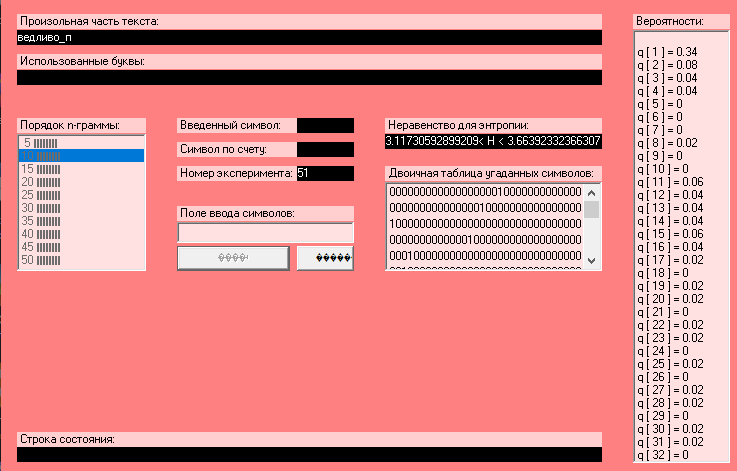
\includegraphics[width=.98\textwidth]{pics/pink1.png}

%\caption{}
\label{fig:overleaf}
\end{figure}

\begin{figure}[h!]
\centering
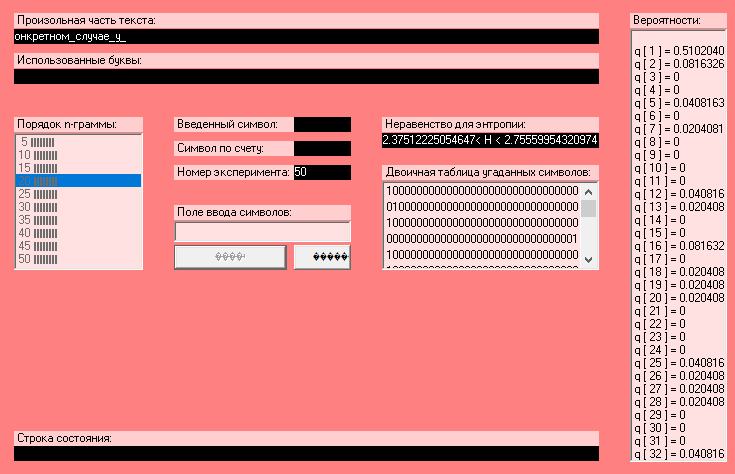
\includegraphics[width=.98\textwidth]{pics/pink2.png}

%\caption{}
\label{fig:overleaf}
\end{figure}

\begin{figure}[h!]
\centering
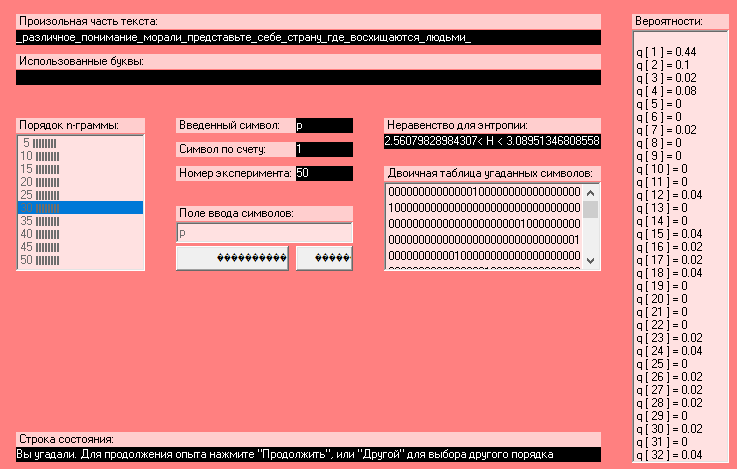
\includegraphics[width=.98\textwidth]{pics/pink3.png}

%\caption{}
\label{fig:overleaf}
\end{figure}


\section{Висновок}
Під час виконання даної лабораторної роботи я навчився вимірювати частоти символів та
біграм у тексті, визначати ентропію. Також, я навчився визначати надлишковість мови.
% \chapter{Название лабораторной работы}

\section{Цель работы}
Здесь приводится формулировка цели лабораторной работы. Формулировки цели для каждой лабораторной работы приведены в методических указаниях. 
В~курсе <<Языки и методы программирования>> используются методические указания \cite{gutgut:1, gutgut:2}.

Цель данного шаблона "--- максимально упростить подготовку отчётов по лабораторным работам в системе \href{https://ru.wikipedia.org/wiki/LaTeX}{\LaTeXe}. 
Модифицируя данный шаблон, студенты смогут без труда подготовить <<стильный>> и качественный (с точки зрения оформления и набора) отчёт по лабораторным работам, а также познакомиться с основными возможностями \LaTeXe, которые безусловно пригодятся при подготовке курсовых и дипломных проектов, оформлении научных статей, магистерских и даже кандидатских диссертаций. 
Для уверенного и <<продвинутого>> владения этой системой настоятельно рекомендуется ознакомиться хотя бы с~одной из этих книг \cite{latex:b1,latex:b2,latex:b3}, которые можно найти в электронном виде в сети Internet или спросить у преподавателя. 
Также можно пользоваться любыми материалами, найденными в сети.

\section{Задание}
Здесь приводится описание задания в соответствии с~рекомендациями методического пособия и~выданным вариантом~\cite{gutgut:1, gutgut:2}.

Студентам предлагается работать с издательской системой \LaTeXe, установленной не на настольном компьютере, а~в~облачном сервисе \href{http://www.overleaf.com}{Overleaf}. 
Это связано с~тем, что пользователю незнакомому с~\LaTeX\ порой весьма трудно самостоятельно установить, настроить и начать работать с этой системой.
Сервис \href{http://www.overleaf.com}{Overleaf} имеет удобный и понятный интерфейс, в нём всё работает <<из коробки>>.

Для начала работы с сервисом \href{http://www.overleaf.com}{Overleaf}  необходимо зарегистрироваться одним из следующих способов: 
\begin{itemize}
\item с помощью аккаунта \href{https://www.overleaf.com/users/auth/google_oauth2?intent=sign_up?ref=21785d9c7b53}{Google};
\item с помощью аккаунта \href{https://www.overleaf.com/users/auth/twitter?intent=sign_up?ref=21785d9c7b53}{Twitter}
\item или с помощью регистрации через  \href{https://www.overleaf.com/signup?ref=21785d9c7b53}{электронную почту}.
\end{itemize}

После регистрации можно открыть этот шаблон по ссылке \url{https://www.overleaf.com/read/sqvxbnhgxxdm} и начать оформлять отчёт по лабораторным работам.
Язык проверки орфографии "--- единственное, что следует изменить в~настройках этого сервиса: \href{https://www.overleaf.com/users/edit#!accountsettings}{Default Spell Check Language (for new projects)}.

На рис.~\ref{fig:overleaf} представлен  экран с тулбаром сервиса Overleaf.
Блок \colorbox{ForestGreen}{\color{white}\verb"PROJECT"}, предназначен для управления файлами проекта, в частности можно добавить и изменить файлы 
\fcolorbox{black}{lightgray}{\color{ForestGreen}Add files...}.
При работе с сервисом рекомендуется использовать режим \colorbox{ForestGreen}{\color{white}\texttt{Source}}, а не
\texttt{Rich Text}.

\begin{figure}[h!]
\centering
\includegraphics[width=.98\textwidth]{overleaf}

\caption{Экран с тулбаром сервиса Overleaf}
\label{fig:overleaf}
\end{figure}

\section{Основная часть}

\subsection{Теоретическая часть}

Здесь приводятся теоретические сведения, необходимые для выполнения соответствующей лабораторной работы: описываются методы решения поставленной задачи, используемые подходы, алгоритмы.

Преимущество \LaTeX{а} перед другими системами в том, что Вы можете набирать свой текст не задумываясь об оформлении. 
Система \LaTeXе\ всё сделает сама в~лучшем виде согласно настройкам, заданным в преамбуле документа, ведь создатель \TeX{а}  не кто иной, как \href{https://ru.wikipedia.org/wiki/%D0%9A%D0%BD%D1%83%D1%82,_%D0%94%D0%BE%D0%BD%D0%B0%D0%BB%D1%8C%D0%B4_%D0%AD%D1%80%D0%B2%D0%B8%D0%BD}{Дональд Кнут}, 
а макропакет \LaTeX\ разработал \href{https://ru.wikipedia.org/wiki/%D0%9B%D1%8D%D0%BC%D0%BF%D0%BE%D1%80%D1%82,_%D0%9B%D0%B5%D1%81%D0%BB%D0%B8}{Лесли Лэмпорт}.

Набор текста, формул и таблиц как правило не вызывает проблем, но в~первое время рекомендуется просматривать уже указанные книги~\cite{latex:b1,latex:b2,latex:b3}, написанные настоящими \href{https://ru.wikipedia.org/wiki/%D0%93%D1%83%D1%80%D1%83_(%D0%B7%D0%BD%D0%B0%D1%87%D0%B5%D0%BD%D0%B8%D1%8F)}{гуру} \LaTeX{а}.

\subsection{Листинг программы}

Листинг программы оформляется с помощью пакета \verb"listings". 
Документация по этому пакету очень обширная, её можно найти по ссылке \url{http://mirrors.ctan.org/macros/latex/contrib/listings/listings.pdf}.
Рекомендуется использовать настройки пакета уже прописанные в данном шаблоне в~преамбуле документа. 
Ниже представлен листинг программы~\ref{listing1} для чтения типизированного файла, взятый из методического пособия~\cite{gutgut:1}, оформленный в~соответствии с прописанными настройками.

\begin{lstlisting}[language=Pascal]
const
	Nmax = 10;
type
	TCircle = record
		x, y, R : integer;
		color : string[20];
	end;
var
	W : array[1..Nmax] of TCircle;
	i, N, min, max : integer;
	f : file of TCircle;
begin
	// открываем файл для чтения
	Assign(f, '0.dbf'); Reset(f);
	N := FileSize(f);;
	for i:=1 to N do begin
		Read(f,W[i]);
	end;
	Close(f);
	max := -MaxInt;
	min := MaxInt;
	for i:=1 to N do begin
		if (W[i].color='зелёный') and (W[i].R>max) then max := W[i].R;
		if (W[i].color='красный') and (W[i].R<min) then min := W[i].R;
  	end;
  	if max = -MaxInt then Writeln('Зелёных кругов нет')
  		else Writeln('Радиус самого большого зелёного круга = ', max);
	if min = MaxInt then Writeln('Красных кругов нет')
		else Writeln('Радиус самого маленького красного круга = ', min);
end.
\end{lstlisting}

В случае, если для выполнения поставленного задания необходимо написать две программ, то приводятся листинги обеих программ.

При необходимости даются комментарии к листингам. Например, в листинге~\ref{listing1} в разделе типов задаётся тип \verb"TCircle", который используется для хранения данных:
\begin{verbatim}
type
	TCircle = record
      x, y, R : integer;
      color : string[20];
    end;
\end{verbatim}

\subsection{Полученные результаты и их анализ}

Здесь кратко описываются итоги проделанной работы, приводится анализ полученных результатов.

Здесь могут содержаться листинги входных и выходных файлов, приводиться таблицы и рисунки, используемые при анализе.

Пример оформления таблицы представлен ниже (см. табл.~\ref{tabl:1}). Она взята из указанного уже методического пособия~\cite{gutgut:1}.

\begin{center}
\begin{table}[h!]
\centering
\caption{Исходные данные для рассматриваемой задачи}
\label{tabl:1}
\begin{tabular}{|c|c|c|c|c|}
\hline
Номер &~~~~$X$~~~~ &~~~~$Y$~~~~&~~~~$R$~~~~&~~~~Цвет~~~~\\
\hline
1 &	100  &	170 & 30 & \color{red} красный\\
2 &	100  &	90	& 60 & \color{yellow} жёлтый\\
3 &	230  &	250	& 50 & \color{blue} синий\\
4 &	130  &	240 & 60 & \color{green} зелёный\\
5 & 300  &	130 & 30 & \color{green} зелёный\\
6 &	200  &	150	& 90 & \color{red} красный\\
\hline
\end{tabular}
\end{table}
\end{center}

Как отмечалось выше, рисунки также могут быть вставлены в отчёт, если они необходимы. См., например, рис.~\ref{fig:1}.

\begin{figure}[h!]
\centering
\includegraphics[scale=1.0]{img33892}

\caption{Задание к одному из вариантов, взятое из методических указаний~\cite{gutgut:2}}
\label{fig:1}
\end{figure}

Подробную информацию о том, как вставлять рисунки и таблицы в документ, также можно найти в уже упоминавшейся литературе~\cite{latex:b1,latex:b2,latex:b3}. 

\section{Выводы}
Здесь кратко описываются итоги проделанной работы.

В настоящем шаблоне заложены основы продуктивной работы в системе \LaTeXe.  Конечно в столь кратком изложении не возможно показать всю мощь и красоту \LaTeX{а}. 
<<Нужно сказать, что \LaTeX\ является \href{https://ru.wikipedia.org/wiki/%D0%9F%D0%BE%D0%BB%D0%BD%D0%BE%D1%82%D0%B0_%D0%BF%D0%BE_%D0%A2%D1%8C%D1%8E%D1%80%D0%B8%D0%BD%D0%B3%D1%83}{Turing complete language}, то есть на нем можно писать любые программы. Например, можно написать \href{http://tug.org/TUGboat/tb11-3/tb29greene.pdf}{интерпретатор Бейсика}, \href{http://en.literateprograms.org/Turing_machine_simulator_%28LaTeX%29}{симулятор машины Тьюринга}, 
\href{http://www.thole.org/manfred/apfel/}{Mandelbrot with LaTeX} и \href{http://stackoverflow.com/questions/2968411/ive-heard-that-latex-is-turing-complete-are-there-any-programs-written-in-late}{другие программы}. То есть на латехе можно писать что угодно.>>

\footnote{Фраза взята вот отсюда: \url{http://mydebianblog.blogspot.ru/2013/12/latex.html}.}

\vfill
\centerline{\Huge Happy \TeX{ing}!}
\vfill
 %Отчёт к каждой работе оформляется в отдельном файле

% Список литературы
% Для отчёта он не обязателен

%\begin{thebibliography}{9}
%\bibitem{gutgut:1} 
%Гутман~Г.~Н. Лабораторные работы по курсу <<Языки и методы программирования>>. URL: \url{http://pm.samgtu.ru/sites/pm.samgtu.ru/files/materials/osnovy_inf/yamp2.doc}

%\end{thebibliography}

\end{document}